% ============================================================
%  Capítulo 6 — Experimentos e Resultados
% ============================================================
\chapter{EXPERIMENTOS E RESULTADOS}
\label{cap:experimentos}

\section{Configuração experimental}
\label{sec:exp-config}

\subsection{Features}
\label{sub:exp-features}

Todos os classificadores utilizam exclusivamente a coluna \texttt{ir\_tokens} do
dataset traduzido como entrada. Nenhuma feature de metadados é utilizada, nome
da função, URL do script, identificador de motor ou posição no código-fonte são
deliberadamente excluídos. Esse isolamento garante que os resultados meçam a
capacidade discriminativa dos bytecodes em si, sem dependência de informações de
contexto que podem não estar disponíveis em cenários de implantação.

A representação de entrada varia por família de modelos, como demonstrado na Tabela~\ref{tab:features}.

\begin{table}[htb]
\centering
\caption{Representação de entrada por família de modelos}
\label{tab:features}
\begin{tabular}{l p{6cm} l}
\toprule
\textbf{Família} & \textbf{Representação} & \textbf{Dimensão} \\
\midrule
RF, SVM, LightGBM & TF-IDF esparso sobre tokens de RI & 136 / 4.723 / 50.631 \\
Transformer (v.1)  & Embeddings FastText 128-dim fixos, seq.\ até 512 tokens & 128 por posição \\
Transformer (v.2)  & Embeddings treináveis 128-dim, seq.\ até 512 tokens & 128 por posição \\
\bottomrule
\end{tabular}

\fonte{Elaborada pelo autor.}
\end{table}

\subsection{Divisão treino/teste}
\label{sub:exp-split}

Os experimentos binários e multilabel utilizam a divisão descrita no
Capítulo~\ref{cap:dataset} (Tabela~\ref{tab:split}: 30.115~FP treino, 7.529~FP
teste). O experimento de modelo conjunto cross-engine
(Seção~\ref{sec:crossengine}) usa uma amostra combinada de ambos os motores
sobre o mesmo conjunto de sites, cujos totais de FP são maiores por incluir
registros independentes de cada motor (Tabela~\ref{tab:split-exp}). O experimento
de transferência zero-shot (Seção~\ref{sub:zeroshot}) usa subconjuntos por motor
do dataset, separados por engine antes da amostragem. A estratificação é feita sobre \texttt{is\_fp} em todos os
casos.

\begin{table}[htb]
\centering
\caption{Divisão treino/teste: experimento cross-engine (modelo conjunto)}
\label{tab:split-exp}
{\footnotesize
Os totais de funções FP (33.087 treino, 8.272 teste) correspondem à amostra do
experimento cross-engine e excedem os 37.644 reportados no
Capítulo~\ref{cap:dataset} por incluir registros independentes de ambos os
motores coletados sobre o mesmo conjunto de sites. O número total de linhas
(525.810) é mantido igual à divisão padrão por sub-amostragem proporcional
dos negativos.
}

\bigskip
\begin{tabular}{lrr}
\toprule
\textbf{Partição} & \textbf{Linhas} & \textbf{FP} \\
\midrule
Treino & 420.648 & 33.087 \\
Teste  & 105.162 &  8.272 \\
\bottomrule
\end{tabular}

\fonte{Elaborada pelo autor.}
\end{table}

\subsection{Métricas}
\label{sub:exp-metricas}

Para a tarefa binária (\texttt{is\_fp}), reportam-se precisão, revocação e F1
sobre a classe positiva após ajuste de limiar (threshold tuning) no conjunto
de teste. O limiar é varrido em passos de 0,05 entre 0 e 1; o valor que maximiza o
F1 é selecionado. Para modelos com limiar padrão (RF), o limiar 0,50 é mantido.

Para a tarefa multilabel, reporta-se o F1 por rótulo e o macro-F1 (média não
ponderada entre os sete rótulos). O macro-F1 penaliza igualmente rótulos raros e
comuns, refletindo a dificuldade total da tarefa.

Para os experimentos cross-engine, reportam-se precisão, revocação e F1 por motor,
mais a média ponderada pelo suporte FP de cada motor.

\subsection{Hiperparâmetros dos modelos principais}
\label{sub:exp-hp}

\textbf{Random Forest (binário):} 200 árvores, balanceamento por subamostragem
por árvore (\textit{balanced\_subsample}), mínimo de 5 amostras por folha.

\textbf{LightGBM (binário):} 500 estimadores, taxa de aprendizado 0,05, 127
folhas por árvore, balanceamento automático de classes, subamostragem de 80\%
de linhas e colunas. Variante com contexto iterativo (iter.~2 e~3): 1.000
estimadores, razão de negativos por positivo $r = 7$.

Hiperparâmetros dos modelos adicionais (SVM, BiLSTM, Transformer, variantes
multilabel) são descritos na Seção~\ref{sec:adicionais}.

\subsection{Ambiente computacional}
\label{sub:exp-ambiente}

Os experimentos com LightGBM, Random Forest, SVM e o benchmark de inferência
foram executados em um notebook com processador Intel Core i7-12700H (20
threads), 16~GB de RAM, sob Fedora Linux~43. O treinamento do Transformer foi
realizado no cluster SLURM \textit{blaise} (PCAD/UFRGS), equipado com 4
GPUs Tesla P100-SXM2.

%, , , , , , , , , , , , , , , , , , , --
\section{Modelo base: LightGBM com bigrams}
\label{sec:baseline}

A Tabela~\ref{tab:bin} e a Figura~\ref{fig:f1-progressao} apresentam os resultados
da linha principal, do piso de unigrams à inferência iterativa com contexto de
script, permitindo acompanhar cada passo de ganho antes de introduzir o seguinte. O modelo oracle
(F1~=~0,928), que usa rótulos reais como features de contexto e não é implantável,
é discutido separadamente na Seção~\ref{sec:oracle}.

\begin{table}[htb]
\centering
\caption{Classificadores binários, linha principal (\texttt{is\_fp})}
\label{tab:bin}
{\footnotesize
Divisão 80/20 estratificada, semente~42. Dataset: 68M funções, 37.644 FP.
$\dagger$ByteDefender: valor reportado sobre bytecodes brutos V8, motor único.
$\P$Inferência iterativa sem rótulos oracle: contagens previstas em três limiares
($p{>}0{,}30$; $p{>}0{,}50$; $p{>}0{,}70$) e tamanho de script, recomputadas a
cada iteração. As variantes iter.~2 e iter.~3 ($\P$) usam $r = 7$; a variante de
duas passagens usa $r = 10$. O conjunto de treinamento menor de iter.~2 e iter.~3
(com $r = 7$) reduz o número de bigramas TF-IDF retidos acima da frequência mínima,
explicando a contagem de features inferior (4.574) em relação à variante de duas
passagens (4.726, treinada com $r = 10$).
}
\bigskip
{\small
\begin{tabularx}{\linewidth}{p{3.2cm}|X|r|r|r|r|l}
\toprule
\textbf{Modelo} & \textbf{Features} & \textbf{\# feat.} & \textbf{P} & \textbf{R} & \textbf{F1} & \textbf{Limiar} \\
\midrule
RF (unigrams)
  & TF-IDF unigrams
  &    136 & 0,834 & 0,835 & 0,834 & 0,50 \\[2pt]
LightGBM (bigrams)
  & TF-IDF bigrams
  &  4.723 & 0,888 & 0,802 & 0,843 & 0,80 \\[2pt]
LightGBM (trigrams)
  & TF-IDF trigrams
  & 50.631 & 0,885 & 0,809 & 0,845 & 0,80 \\[2pt]
LightGBM + densidade
  & TF-IDF bigrams + densidade de script
  &  4.724 & 0,883 & 0,825 & 0,853 & 0,80 \\[2pt]
LightGBM + duas passagens$\P$
  & + dens.\ + contagem FP prev.\ + tam.\
  &  4.726 & 0,901 & 0,848 & 0,874 & 0,80 \\[2pt]
LightGBM + iter.\ 2$\P$
  & + dens.\ + 3 cont.\ limiares + tam.\
  &  4.574 & 0,917 & 0,886 & 0,901 & 0,70 \\[2pt]
\textbf{LightGBM + iter.\ 3}$\P$
  & \textbf{idem iter.\ 2}
  & \textbf{4.574} & \textbf{0,934} & \textbf{0,876} & \textbf{0,904} & \textbf{0,80} \\[2pt]
ByteDefender$\dagger$ (motor único)
  & Bytecodes brutos V8
  & --- & --- & --- & $\approx$0,950 & --- \\
\bottomrule
\end{tabularx}
}% end \small
\fonte{Elaborada pelo autor.}
\end{table}

\begin{figure}[htb]
\centering
\caption{Progressão do F1 binário: do modelo base à inferência iterativa}
\label{fig:f1-progressao}
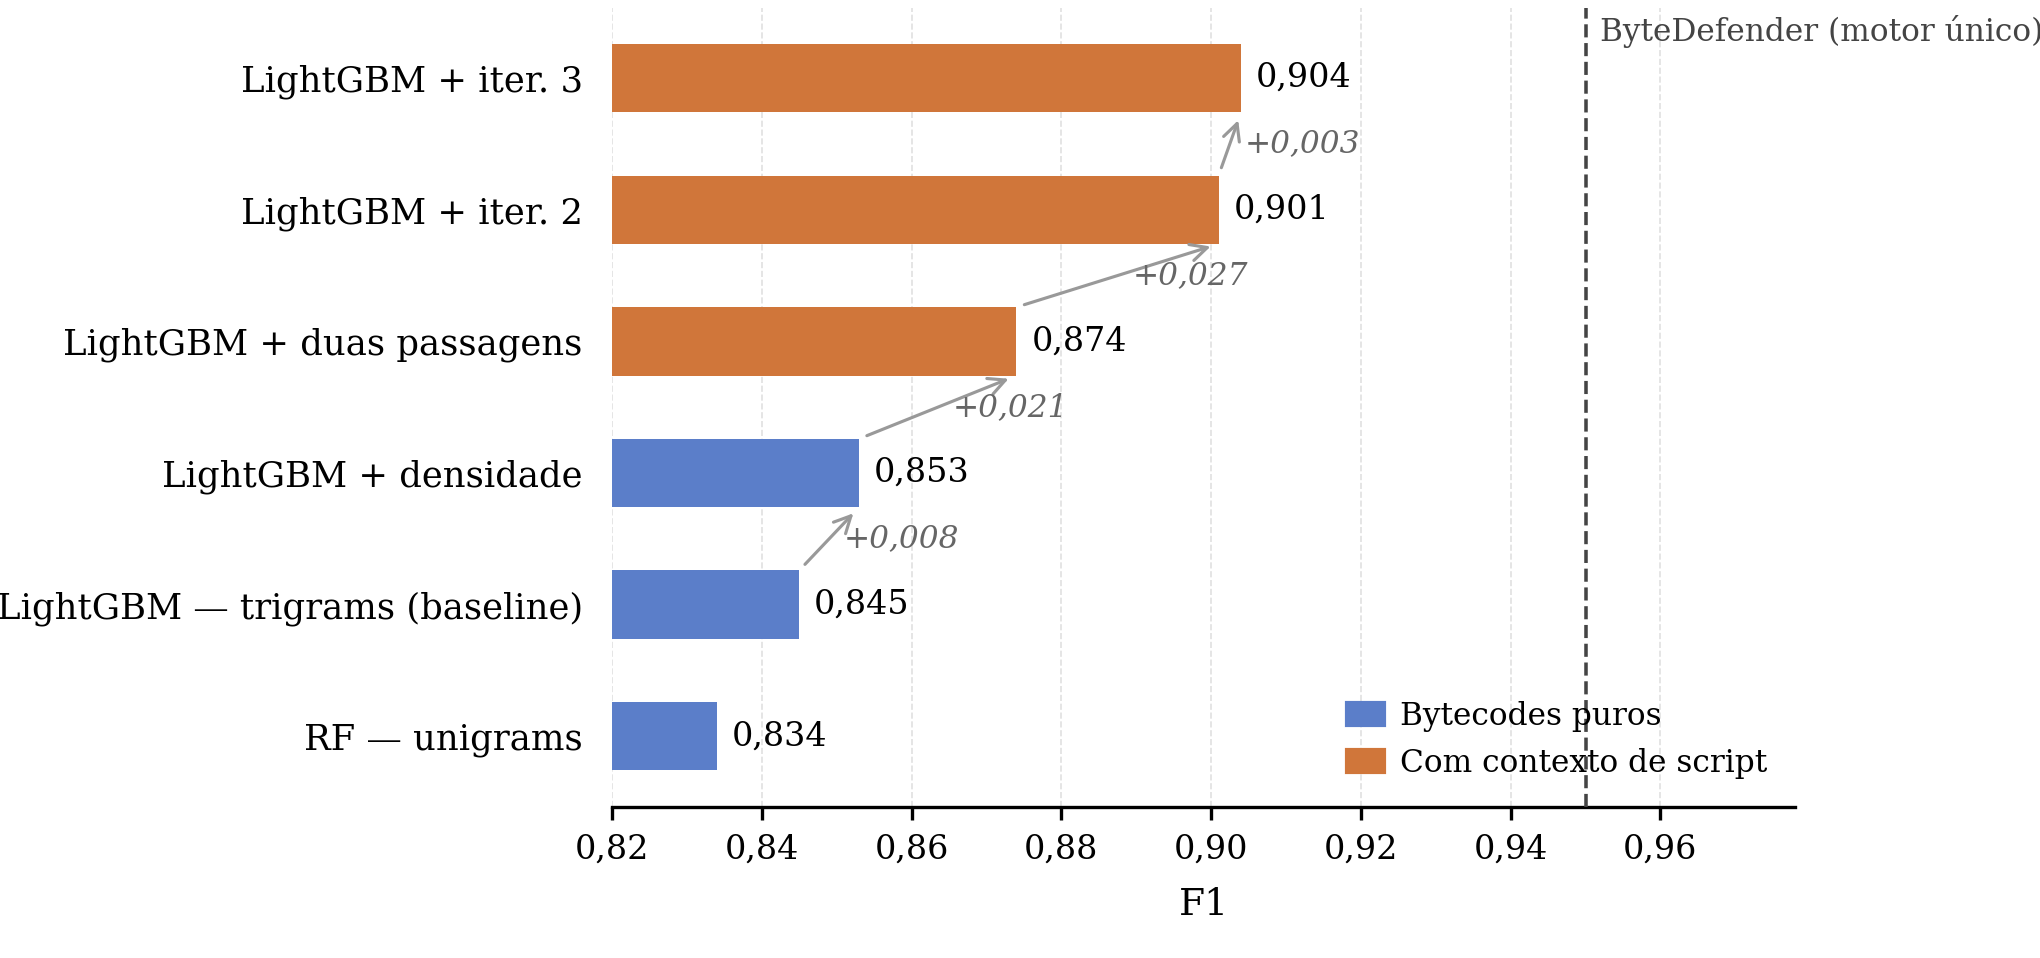
\includegraphics[width=0.88\linewidth]{fig_f1_progression}
\fonte{Elaborada pelo autor.}
\end{figure}

\textbf{RF como piso interpretativo.} O RF com unigrams (136~features) atinge
F1~=~0,834, confirmando que as frequências de tokens individuais da RI já codificam
sinal discriminativo substancial. Funções de fingerprinting são
caracterizadas por alta frequência de tokens de acesso a propriedades
(\texttt{get\_keyed\_prop}, \texttt{get\_named\_prop}) e de chamadas de método
(\texttt{call\_func}); esses padrões são suficientemente distintos para separar a
maioria dos positivos com um modelo simples de 136~features. Qualquer modelo mais
complexo deve superar esse piso para justificar a complexidade adicional.

\textbf{LightGBM com trigrams confirma o teto de n-gramas.} O LightGBM com trigrams
TF-IDF atinge F1~=~0,845 (P~=~0,885, R~=~0,809, limiar~=~0,80), ganho de apenas +0,002
sobre os bigrams apesar de 10,7$\times$ mais features (50.631 vs.\ 4.723). Esse plateau
indica que o espaço de n-gramas sobre 145 tokens está essencialmente exaurido nos bigrams;
os enriquecimentos de features subsequentes partem do modelo de bigrams (F1~=~0,843) como
referência, buscando superar o teto de bytecodes puros de $\approx$F1~0,85. A análise
detalhada está na Seção~\ref{sec:adicionais}.

%, , , , , , , , , , , , , , , , , , , --
\section{Contexto de script e inferência iterativa}
\label{sec:iterativo}

A principal limitação do LightGBM baseline é a classificação em isolamento: cada
função é avaliada independentemente, sem informação sobre o script em que está
inserida. Funções de fingerprinting tendem a co-ocorrer no mesmo script, uma biblioteca como \texttt{fingerprintjs} empacota dezenas de funções
especializadas em um único arquivo, e bibliotecas menores de WebGL ou áudio
raramente aparecem em scripts de propósito geral. Incorporar essa co-ocorrência sem
usar rótulos externos é o objetivo das três etapas desta seção.

\textbf{Densidade de script.} O primeiro estágio adiciona como feature a densidade
média de fingerprinting do script: a fração de funções no mesmo arquivo com
probabilidade prevista acima de 0,5, calculada com o LightGBM baseline em uma
passagem prévia sobre o dataset completo. Nenhum rótulo real é consultado. O
resultado é F1~=~0,853 (+0,008 sobre o baseline de trigrams, +0,019 sobre o RF,
P~=~0,883, R~=~0,825, limiar~=~0,80). O ganho de divisão dessa única feature (2.949)
é o maior de qualquer feature individual do modelo com densidade, superando qualquer bigram
TF-IDF \emph{nesse mesmo modelo}, e confirma que a co-ocorrência de script é um sinal genuinamente
informativo, irredutível à frequência de tokens por função. Nota: os ganhos de divisão
reportados aqui (escala de unidades a milhar) não são diretamente comparáveis com
os da Tabela~\ref{tab:features-imp}, que correspondem ao modelo de bigrams sem feature
de densidade; ao adicionar a densidade, o modelo redistribui parte substancial do
ganho para essa nova feature, reduzindo os ganhos individuais dos bigrams. Destaca-se ainda que
esse modelo usa apenas bigrams TF-IDF mais a feature de densidade (4.724 features
no total, cf.\ Tabela~\ref{tab:bin}), mas supera o baseline de trigrams
(50.631~features), demonstrando que uma feature de contexto de script vale mais do
que 10$\times$ mais n-grams.

\textbf{Inferência em duas passagens.} O segundo estágio enriquece o vetor de
contexto: além da densidade, acrescenta a contagem absoluta de funções com
probabilidade prevista acima de~0,5 e o logaritmo do tamanho total do script.
A motivação é que a densidade relativa e a contagem absoluta capturam aspectos
complementares: um script com 3 de 5 funções previstas como FP
(densidade~=~0,60) transmite sinal distinto de um com 3 de 300
(densidade~=~0,01), mesmo que a contagem absoluta seja idêntica. O resultado é
F1~=~0,874 (+0,021 sobre a densidade, P~=~0,901, R~=~0,848, limiar~=~0,80).

\textbf{Inferência iterativa com contagens em múltiplos limiares.} O terceiro
estágio substitui a contagem única por três contagens em limiares distintos
($p{>}0{,}30$; $p{>}0{,}50$; $p{>}0{,}70$), capturando a forma da
distribuição de probabilidades dentro de cada script. Um script com muitas funções
classificadas a $p \approx 0{,}4$ (positivos suaves) é qualitativamente diferente
de um com poucas funções a $p{>}0{,}70$ (positivos de alta confiança), mesmo que a
densidade seja semelhante. Com \texttt{neg\_ratio} = 7 e 1.000 árvores, a iteração~2 atinge
\textbf{F1~=~0,901} (P~=~0,917, R~=~0,886, limiar~=~0,70). Os split gains das features de contexto dominam todas as demais: 4.952
(densidade), 4.410 (logaritmo do tamanho), 4.149 (contagem $p{>}0{,}30$),
3.944 (contagem $p{>}0{,}70$), 3.391 (contagem $p{>}0{,}50$).

Um ciclo adicional de auto-melhora, recomputando as contagens com o modelo da
iteração~2 e retreinando com os mesmos parâmetros, produz
\textbf{F1~=~0,904} (P~=~0,934, R~=~0,876, limiar~=~0,80, iter.~3). A progressão
por iteração é +0,021, +0,027, +0,003, confirmando convergência gradual com
retornos decrescentes a partir da iteração~2. O modelo da iteração~3 é o
\textbf{resultado implantável principal deste trabalho}: F1~=~0,904 sem nenhum
rótulo prévio, usando apenas predições do próprio modelo iteradas sobre o corpus
completo.

%, , , , , , , , , , , , , , , , , , , --
\section{Generalização cross-engine}
\label{sec:crossengine}

\subsection{Transferência zero-shot}
\label{sub:zeroshot}

O experimento de transferência zero-shot treina o LightGBM de bigrams sobre
funções de um único motor (conjunto completo de dados disponível para esse motor) e
avalia sobre o conjunto completo do outro motor. Nenhum dado do motor de teste está
disponível durante o treinamento.

\begin{table}[htb]
\centering
\caption{Transferência zero-shot (LightGBM bigrams, sem dados do motor de teste)}
\label{tab:zeroshot}
{\small
\begin{tabular}{lrrrrrrl}
\toprule
\textbf{Treino $\to$ Teste} & \textbf{Tam.\ treino} & \textbf{Tam.\ teste} & \textbf{FP teste} & \textbf{Limiar} & \textbf{P} & \textbf{R} & \textbf{F1} \\
\midrule
Chromium $\to$ Firefox & 191.565 & 296.610 & 27.312 & 0,05 & 0,093 & 0,363 & \textbf{0,149} \\
Firefox $\to$ Chromium & 296.965 & 191.692 & 14.047 & 0,05 & 0,123 & 0,341 & \textbf{0,180} \\
\bottomrule
\end{tabular}
}% end \small
{\footnotesize As leves diferenças entre o tamanho de treino e de teste de um mesmo
motor (ex.: Firefox treino 296.965 vs.\ teste 296.610) decorrem da estratificação
por \texttt{is\_fp} realizada independentemente em cada direção do experimento.}

\fonte{Elaborada pelo autor.}
\end{table}

Os limiares de 0,05 revelam o estado de colapso do classificador: para obter
qualquer revocação razoável, é necessário aceitar um número massivo de falsos
positivos. A precisão de 0,093--0,123 corresponde a aproximadamente 1 verdadeiro
positivo para cada 7--10 alarmes falsos. O F1 de 0,149--0,180 confirma que a
transferência zero-shot falha completamente.

A causa é estrutural: TF-IDF sobre bigrams captura padrões de sequência locais.
Embora ambos os motores compartilhem o mesmo vocabulário de tokens de RI após a
tradução, as distribuições de n-grams diferem sistematicamente: V8 e
SpiderMonkey compilam a mesma operação JavaScript em ordens de tokens distintas
(ver Seção~\ref{sec:ir-motivacao}). O modelo aprende limites de decisão moldados
pela distribuição de bigrams do motor de origem; esses limites não se transferem.

\subsection{Modelo conjunto por motor}
\label{sub:conjunto}

O experimento de modelo conjunto treina um único LightGBM de bigrams sobre a
amostra mista (dados de ambos os motores), usando a divisão cross-engine 80/20
estratificada descrita na Tabela~\ref{tab:split-exp} (33.087~FP treino, 8.272~FP
teste — totais maiores que os 37.644 da divisão padrão por incluir registros
independentes de cada motor). O conjunto de teste é então filtrado por
motor para avaliar o desempenho por engine separadamente, sem vazamento de dados de
treinamento.

\begin{table}[htb]
\centering
\caption{Modelo conjunto bigrams: avaliação por motor no conjunto de teste (LightGBM bigrams)}
\label{tab:conjunto}
\begin{tabular}{lrrrr}
\toprule
\textbf{Motor} & \textbf{P} & \textbf{R} & \textbf{F1} & \textbf{Suporte FP} \\
\midrule
Chromium (V8)            & 0,933 & 0,828 & \textbf{0,877} & 2.873 \\
Firefox (SpiderMonkey)   & 0,864 & 0,830 & \textbf{0,847} & 5.399 \\
\midrule
\textbf{Média ponderada} & 0,888 & 0,829 & \textbf{0,857} & 8.272 \\
\bottomrule
\end{tabular}

\fonte{Elaborada pelo autor.}
\end{table}

A média ponderada de 0,857 coincide exatamente com o F1 global do modelo
(Tabela~\ref{tab:conjunto}), confirmando que a divisão de teste está balanceada entre os
motores e que a avaliação é internamente consistente, não há viés de amostragem
que favorecesse um motor no conjunto de teste global.

O modelo conjunto atinge F1~=~0,877 no Chromium e F1~=~0,847 no Firefox a partir
de um único conjunto de pesos, sem retreinamento por motor. O F1 global de 0,857
corresponde à média ponderada pelo suporte desses dois valores (Tabela~\ref{tab:conjunto}),
confirmando consistência entre a avaliação por motor e a métrica global.
A diferença de $\approx$0,030 entre os motores (0,877 vs.\ 0,847) é consistente com
a maior regularidade estrutural dos bytecodes do V8 (máquina de registradores, sequências
mais compactas) em relação ao SpiderMonkey (máquina de pilha, maior verbosidade), que
produz padrões de n-gramas V8 mais uniformes e portanto mais discriminativos para o
classificador TF-IDF.

Quando o modelo conjunto é aumentado com as mesmas cinco features de contexto
iterativo da Tabela~\ref{tab:bin} (densidade de script, três contagens por limiar e
tamanho), o desempenho por motor melhora significativamente.

\begin{table}[htb]
\centering
\caption{Modelo conjunto com contexto iterativo (iter~3): avaliação por motor}
\label{tab:conjunto-iter}
{\footnotesize
Avaliado na divisão padrão (Tabela~\ref{tab:split}: 7.529~FP de teste total,
1.521 Chromium + 6.008 Firefox), diferente da divisão cross-engine usada na
Tabela~\ref{tab:conjunto} (8.272~FP). Os suportes por motor diferem entre as
duas tabelas porque os datasets foram construídos com estratégias de amostragem
distintas: a divisão padrão parte do dataset unificado (37.644~FP, razão
Firefox:Chromium de $\approx$4:1 no corpus), enquanto a divisão cross-engine
amostra cada motor independentemente, elevando o total de FP (41.359) e
redistribuindo a proporção relativa entre os motores. A comparação direta
de F1 entre as tabelas é, portanto, aproximada.
}

\bigskip
\begin{tabular}{lrrrr}
\toprule
\textbf{Motor} & \textbf{P} & \textbf{R} & \textbf{F1} & \textbf{Suporte FP} \\
\midrule
Chromium (V8)            & 0,941 & 0,869 & \textbf{0,903} & 1.521 \\
Firefox (SpiderMonkey)   & 0,932 & 0,878 & \textbf{0,904} & 6.008 \\
\bottomrule
\end{tabular}

\fonte{Elaborada pelo autor.}
\end{table}

O modelo iterativo atinge F1~=~0,903 no Chromium e F1~=~0,904
no Firefox (divisão padrão). A homogeneidade entre motores, diferença de apenas 0,001, confirma
que a RI com treinamento conjunto produz representações igualmente úteis para ambos
os engines quando complementadas por contexto de script.

%, , , , , , , , , , , , , , , , , , , --
\section{Importância de features}
\label{sec:features}

A Tabela~\ref{tab:features-imp} apresenta as 15 features de maior ganho de divisão
(split gain) no modelo LightGBM de bigrams. O ganho de divisão mede a
redução total de impureza atribuída a cada feature ao longo de todas as árvores e
divisões do ensemble.

\begin{table}[htb]
\centering
\caption{Top-15 features por ganho de divisão (LightGBM bigrams)}
\label{tab:features-imp}
\begin{tabular}{rlrr}
\toprule
\textbf{Rank} & \textbf{Feature (token ou bigram de RI)} & \textbf{Ganho} & \textbf{Divisões} \\
\midrule
 1 & \texttt{get\_keyed\_prop}                  & 718.016 &  280 \\
 2 & \texttt{load\_closure\_var}                & 249.551 &  787 \\
 3 & \texttt{call\_func get\_keyed\_prop}        & 237.632 &  163 \\
 4 & \texttt{get\_named\_prop}                  & 211.451 &  700 \\
 5 & \texttt{return}                            & 195.687 &  961 \\
 6 & \texttt{call\_func}                        & 166.258 &  669 \\
 7 & \texttt{load\_closure\_var call\_func}     &  83.605 &  241 \\
 8 & \texttt{load\_undefined call\_func}        &  83.188 &  243 \\
 9 & \texttt{pop\_scope}                        &  81.646 &  125 \\
10 & \texttt{call\_func pop}                    &  80.206 &  390 \\
11 & \texttt{store\_closure\_var}               &  79.208 &  356 \\
12 & \texttt{load\_undefined set\_exception}    &  69.639 &   51 \\
13 & \texttt{call\_func store\_local}           &  62.009 &  358 \\
14 & \texttt{load\_global get\_named\_prop}     &  61.085 &  170 \\
15 & \texttt{call\_func return}                 &  59.609 &  351 \\
\bottomrule
\end{tabular}

\fonte{Elaborada pelo autor.}
\end{table}

\textbf{\texttt{get\_keyed\_prop}} lidera com folga (ganho 718.016, quase 3$\times$
o segundo colocado), refletindo o padrão central de fingerprinting: acessar
propriedades indexadas de objetos de API como \texttt{gl.getParameter(pname)} ou
\texttt{screen[prop]}. Esse padrão está presente em todas as sete categorias de
fingerprinting.

\textbf{\texttt{load\_closure\_var}} (ganho 249.551, 787 divisões, o segundo maior
número de divisões na lista, abaixo apenas de \texttt{return} com 961) codifica o uso de closures típico de
bibliotecas de fingerprinting empacotadas em IIFE (Immediately Invoked
Function Expressions): os resultados intermediários são armazenados e recuperados
via variáveis de closure entre funções internas do módulo.

\textbf{Bigrams de acesso-chamada} como \texttt{call\_func get\_keyed\_prop} e
\texttt{load\_closure\_var call\_func} capturam a sequência invoke-then-read:
chamar um método de API e imediatamente ler a propriedade do resultado, padrão
idiomático em WebGL (\texttt{gl.getParameter(...)}) e Canvas
(\texttt{ctx.measureText(...).width}).

\textbf{\texttt{load\_undefined set\_exception}} (rank~12, 51 divisões, alto ganho
por divisão: $\approx$1.366 por divisão) corresponde ao bloco
\texttt{try \{ ... \} catch(e) \{\}} que bibliotecas de fingerprinting usam
para testar a disponibilidade de APIs de forma resiliente entre navegadores. Esse
padrão é altamente discriminativo por seu ganho por divisão elevado, cada vez
que o modelo usa essa feature, ela reduz substancialmente a impureza do nó.

A predominância de tokens de acesso a propriedades (\texttt{get\_keyed\_prop},
\texttt{get\_named\_prop}, \texttt{load\_global get\_named\_prop}) e de chamadas
de função/método (\texttt{call\_func}, \texttt{call\_func get\_keyed\_prop}) na
lista reflete a natureza de fingerprinting: coleta sistemática de
propriedades de objetos de API do browser, encadeada com chamadas que processam ou
armazenam os resultados.

%, , , , , , , , , , , , , , , , , , , --
\section{Experimentos Adicionais}
\label{sec:adicionais}

Esta seção consolida experimentos que complementam a linha principal com contexto
comparativo sobre outras famílias de modelos, variantes de features e o limite
superior oracle.

\subsection{Expansão para trigrams e teto de bytecodes}
\label{sub:trigrams}

Bigrams e trigrams TF-IDF atingem respectivamente F1~=~0,843 e F1~=~0,845
(4.723 vs.\ 50.631 features). O gap entre bigrams e
trigrams (teto de bytecodes puros em $\approx$F1~0,85)
não se fecha ao se acrescentar mais features, e bigrams+densidade supera o baseline
de trigrams com apenas 4.724~features, confirmando a interpretação. O plateau entre bigrams e trigrams é
explicado na Seção~\ref{sec:disc-teto}: os trigrams reexpressam combinações de
bigrams discriminativos sem introduzir informação nova, pois o comportamento de
fingerprinting se concentra em poucos padrões de opcode que já estão cobertos
pelos bigrams retidos.

\subsection{SVM}
\label{sub:svm-exp}

O SVM com gradiente estocástico e perda de dobradiça, calibrado em
probabilidades, sobre TF-IDF de bigrams, atinge F1~=~0,649 (P~=~0,644,
R~=~0,653, limiar~=~0,35), bem abaixo do LightGBM com as mesmas features
(F1~=~0,843) e abaixo até do RF com unigrams (F1~=~0,834). A calibração de
probabilidades introduz ruído nos limiares de decisão, e o gradiente estocástico
com perda de dobradiça produz margens menos estáveis do que o LightGBM com
histogram splitting no regime de alta dimensionalidade esparsa.

\subsection{BiLSTM}
\label{sub:bilstm}

Uma BiLSTM de duas camadas (256 unidades ocultas, embedding $145 \times 64$
RI com separação de aridade descrita na Seção~\ref{sub:aridade},
pooling mean+max) treinada atinge F1~=~0,856 (P~=~0,894,
R~=~0,821, limiar~=~0,95), superior em +0,013~F1 ao LightGBM de bigrams
(F1~=~0,843), mas com modelo substancialmente mais pesado e maior custo de
treinamento. O ganho marginal confirma que a informação sequencial captada pelo BiLSTM
não acrescenta discriminação substancial além do que o TF-IDF de bigrams já codifica;
o vocabulário fechado de 145~tokens limita a vantagem de qualquer representação sequencial.

\subsection{Transformer}
\label{sub:transformer}

\textbf{Versão~1 (FastText fixo, F1~=~0,415):} O Transformer original (2 camadas
de codificador, embeddings FastText 128-dim fixos, Focal Loss, treinado
em 4$\times$ Tesla P100-SXM2) obteve resultado anomalamente baixo. A investigação
identificou três causas: (1)~bug de conversão de tipo nas sequências de entrada;
(2)~Focal Loss instável com vocabulário fechado de 145~tokens; (3)~embeddings
fixos que impedem adaptação ao domínio.

\textbf{Versão~2 (embeddings treináveis, F1~=~0,764):} Corrigidos os três
problemas --- conversão correta de tipos nas entradas, substituição da Focal
Loss por BCE ponderada e embeddings iniciados aleatoriamente e treinados
conjuntamente --- com pooling mean+max em vez de mean-only, o modelo atinge
F1~=~0,764 (P~=~0,817, R~=~0,717, limiar~=~0,85). O gap remanescente em
relação ao LightGBM ($\approx$0,09~F1) reflete uma limitação arquitetural: com
sequências de tokens altamente repetidos (ex.: 50$\times$ \texttt{load\_local} em
uma mesma função), o mecanismo de auto-atenção degenera em bag-of-words,
perdendo a vantagem posicional que o Transformer deveria oferecer.

\subsection{Features estruturais locais}
\label{sub:estrutural}

Seis features escalares derivadas da sequência de tokens de RI — contagem de tokens,
contagem de leituras de propriedades, contagem de chamadas, densidade de leituras
de propriedades, número de tipos distintos e presença de variável de fechamento —
foram acrescentadas ao LightGBM de bigrams. O resultado é F1~=~0,842
(P~=~0,886, R~=~0,801, 4.729 features): ganho nulo ($\approx{-}0{,}001$) em relação
ao baseline de bigrams (F1~=~0,843).
As features estruturais não carregam informação independente porque as frequências
TF-IDF já as codificam implicitamente: uma função densa em tokens \texttt{call\_*}
terá alta frequência nesses unigrams, e o TF-IDF já captura isso como feature
individual.

\subsection{IR com separação de aridade}
\label{sub:aridade}

O dicionário base (Apêndice~\ref{ap:ir-dict}) mantém separação de aridade para
opcodes V8 de chamada de função (\texttt{CALL\_FUNC\_0}, \texttt{CALL\_FUNC\_1},
\texttt{CALL\_FUNC\_2}, \texttt{CALL\_FUNC\_N}, \texttt{CALL\_METHOD\_0},
\texttt{CALL\_METHOD\_1}, \texttt{CALL\_METHOD\_2}, \texttt{CALL\_METHOD\_N}),
refletindo que o V8 emite opcodes distintos conforme o número de argumentos
(\texttt{CallUndefinedReceiver0}, \texttt{CallUndefinedReceiver1}, etc.). Uma
variante experimental colapsa esses oito tokens em dois (\texttt{CALL\_FUNC} e
\texttt{CALL\_METHOD\_N}), na hipótese de que a granularidade de aridade não
acrescentaria discriminação útil. O LightGBM com bigrams sobre essa variante
colapsada (4.623~features) atinge F1~=~0,857, equivalente ao modelo base de bigrams
(4.723~features). A redução no número de features da variante colapsada (4.623 vs.\ 4.723~do modelo base)
é atenuada pelo aumento de frequência dos tokens fundidos, que fazem mais bigramas
superarem o limiar mínimo de frequência (\texttt{min\_df}).
A aridade das chamadas não acrescenta informação discriminativa sobre o tipo de função.

\subsection{Classificadores multilabel}
\label{sec:multilabel}

A Tabela~\ref{tab:multilabel} apresenta os resultados por categoria e o macro-F1
para os três modelos multilabel. O suporte de teste por rótulo reflete a
distribuição apresentada no Capítulo~\ref{cap:dataset}.

\begin{table}[htb]
\centering
\caption{Classificadores multilabel: 7 categorias de fingerprinting}
\label{tab:multilabel}
{\footnotesize
Mesma divisão e features da Tabela~\ref{tab:bin}. Suporte de teste: Canvas~1.635,
Áudio~182, WebRTC~39, Fonte~39, WebGL~2.001, Tela~5.323, Navigator~2.844.
}

\bigskip
\resizebox{\linewidth}{!}{%
\begin{tabular}{lrrrrrrrl}
\toprule
\textbf{Modelo} & \textbf{Canvas} & \textbf{Áudio} & \textbf{WebRTC} & \textbf{Fonte} & \textbf{WebGL} & \textbf{Tela} & \textbf{Navigator} & \textbf{Macro-F1} \\
\midrule
RF (200 árvores, bal.\ por subamostragem) & 0,687 & 0,480 & 0,201 & 0,345 & 0,729 & 0,755 & 0,747 & \textbf{0,564} \\
LightGBM (classificador multirrótulo)      & 0,818 & 0,198 & 0,001 & 0,001 & 0,826 & 0,758 & 0,788 & 0,484 \\
Transformer (Focal Loss)                & 0,204 & 0,075 & 0,017 & 0,013 & 0,288 & 0,279 & 0,320 & 0,171 \\
\bottomrule
\end{tabular}%
}
\fonte{Elaborada pelo autor.}
\end{table}

\textbf{O RF é o melhor modelo multilabel} (macro-F1~=~0,564). A estratégia de
balanceamento por subamostragem por árvore reamostra cada árvore
individualmente, produzindo classificadores por rótulo mais robustos a
desequilíbrios extremos do que a abordagem de pesos globais do LightGBM. O
LightGBM com balanceamento automático de classes colapsa nos rótulos raros: o
classificador WebRTC atinge P~=~0,0007 (F1~=~0,001), predizendo positivo para
quase todas as funções do conjunto de teste. O Transformer com Focal Loss não converge para
representações úteis nos rótulos raros com apenas 39 positivos de teste para os rótulos raros
(WebRTC e Fonte; suporte do conjunto de teste, ver nota da tabela). Para
os rótulos bem suportados (Tela, WebGL, Navigator, Canvas), todos os três modelos
produzem F1 acima de~0,68, confirmando que os bytecodes da RI carregam sinal
multilabel genuíno quando o suporte é adequado. A discussão completa está na
Seção~\ref{sec:disc-raro}.

\subsection{Benchmark de inferência}
\label{sec:inferencia}

\begin{table}[htb]
\centering
\caption{Benchmark de inferência: LightGBM bigrams (CPU, processo único)}
\label{tab:inferencia}
{\footnotesize
$n_{\text{reps}}$: número de repetições para estimativa de média e percentis.
Medições em ambiente quiescente; p99 inclui variação de sistema operacional.
}

\bigskip
{\small
\begin{tabular}{rrrrrrl}
\toprule
\textbf{Lote} & \textbf{$n_{\text{reps}}$} & \textbf{Média (ms)} & \textbf{p50 (ms)} & \textbf{p95 (ms)} & \textbf{p99 (ms)} & \textbf{Por função (µs)} \\
\midrule
    1 & 200 &  3,31 &  2,84 &  4,08 & 18,73 & 3.308 \\
   10 &  20 &  4,19 &  3,31 &  5,74 & 16,23 &   419 \\
  100 &   5 &  9,28 &  8,95 &  9,91 &  9,98 &  92,8 \\
1.000 &   5 & 44,15 & 44,05 & 45,64 & 45,87 & \textbf{44,1} \\
\bottomrule
\end{tabular}
}% end \small
\fonte{Elaborada pelo autor.}
\end{table}

Com lote de 1.000 funções, o modelo classifica a \textbf{44,1~µs por função}
(vazão de $\approx$22.700~funções/segundo). O traço de bytecodes de uma página web
típica, algumas centenas de funções JavaScript, seria classificado em menos
de 15~ms. Com lote unitário, a latência de 3,31~ms é dominada pela construção da
matriz TF-IDF esparsa; em produção, o processamento em lote elimina esse custo
fixo. A discussão de cenários de implantação está na
Seção~\ref{sec:disc-implantacao}.

\subsection{Limite superior oracle}
\label{sec:oracle}

O modelo oracle (LightGBM + bigrams + densidade de script + 6~features estruturais
+ 4~features de contexto de script real) atinge \textbf{F1~=~0,928} (P~=~0,944, R~=~0,912,
limiar~=~0,90). As features de contexto real são: contagem absoluta de funções FP
no mesmo script, contagem total de funções, razão entre elas e logaritmo do
tamanho, calculadas sobre as 68M linhas do dataset antes da divisão
treino/teste, com os rótulos reais.

\textbf{Este resultado não é implantável.} Em produção, os rótulos reais não estão
disponíveis no momento da classificação. O modelo oracle estabelece um
limite superior para sistemas de co-ocorrência de script: o desempenho
atingível se todas as funções vizinhas de um script fossem previamente rotuladas
com perfeição. O modelo iterativo (iter.~3, F1~=~0,904) recupera $\approx$68\%
desse intervalo sem consultar nenhum rótulo real; a diferença remanescente de 0,024
e sua irredutibilidade são analisadas na Seção~\ref{sec:disc-teto}.
